\section{Discussion}
\label{sec:discussion}

We have introduced a new variant of the replicator mutator dynamics
that implements specifically stochastic noise in the form of
confusability of similar states. The probabilities of confusing nearby
similar states is easily implemented in behavioral strategies, but can
also be translated into a mutation matrix for pure strategies. This
allows, in principle, several conceptual interpretations of the \rdd,
on which we will briefly enlarge below in
Section~\ref{sec:model-interpretation}.

Next to this technical contribution, the results of our numerical
simulations also advance our understanding of the possibility of
evolving regular and efficient categories despite their (higher-order)
vagueness. Section~\ref{sec:relat-with-prev} zooms in on the relation
with closely related accounts once more, to delineate the present
approach more precisely.

\subsection{Model interpretation}
\label{sec:model-interpretation}

We mentioned in passing in Section~\ref{sec:repl-diff-dynam-1} that
adding diffusion to other discrete-time evolutionary dynamics that
operate on behavioral strategies is entirely straightforward. We
could, for instance, easily diffuse the outcome of a best-response
dynamic at each time step. That would make sense if we thought of
agents as prone to confusing similar states that are otherwise
rational optimizers of behavior. The reason that we chose the
replicator dynamics to combine with diffusion is twofold. A minor
reason is that it makes for a conceptually interesting link with the
replicator mutator dynamics. A more important reason is that the
replicator dynamic is especially versatile and non-committal about
what the exact process of adaption is that is being modelled.

Originally the \rd was introduced as mathematical model of evolution
under asexual reproduction, motivated by concepts from the theory of
natural selection \citep{TaylorJonker1978:Evolutionary-St}. The most
conservative interpretation of the \rdd in our present context is thus
a biological one: we can imagine signaling strategies as innate or
fixed behaviorial tendencies of organisms, steps in the evolutionary
process as successive generations, and selection as capturing the
reproductive advantage of fitter individuals. This interpretation,
strictly speaking, requires formalization in terms of mixed strategies
via the \rmd, and possibly also a symmetrizing of the game, so that
every agent is assumed to have a unique sender and receiver role at
the same time the is bequeathed onto the next generation. Diffusion,
in this context, could be either of two things. It could be
differential mutation probabilities in line with other interpretation
of mutation in the \rmd
\citep[e.g.][]{NowakKomarova2001:Evolution-of-Un,KomarovaNiyogi2001:The-Evolutionar}:
pure strategies are not faithfully reproduced, and mistakes in
bequeathing pure strategies are more likely if they result from the
confusion of similar states. Another possible biological
interpretation of the \rdd, is that inheritance is faithful, but
strategies are noisily realized. Strategies are not necessarily
selected for what they are, but rather for how they are realized, once
noise is factored in. 

But the replicator dynamic is not only a model of biological
evolution. It can also be interpreted as a high-level description of
the likely development of other behavioral adaptation processes, like
differential imitation and cultural evolution in general
\citep[see][for various derivations of the
\rd]{Sandholm2013:Population-Game}. Under this interpretation, the \rd
is consistent with the idea that what is subject to the evolutionary
forces are not organisms but behavior: individuals can adapt their
behavior to the perceived environment or adopt strategies from other
individuals. Fitness captures the success of behavioral patterns,
which in the case of language can be thought of in terms of
communicative success.  Differential reproduction represents the
tendency of more successful strategies to be more likely adopted by
individuals, be it through imitation or some learning procedure within
the population.  

Under this non-biological interpretation, we have again two options of
picturing what diffusion is, similar to the biological cases
before. One possibility is that diffusion is noise in the adoption of
strategies, say, by conditional imitation, of strategies by other
signalers. Another possibility is that diffusion is again noise on the
realization of strategies: while behavior is optimized to be efficient
(be it due to learning, introspection or imitation), realization of
strategies is bound to be noisy due to confusability of similar
states. 

We believe that all of the four mentioned interpretations are, on
first approximations, feasible conceptualizations of the \rdd, and
that it is a good thing to know of a working account of vague
signaling that sketches where fitness-based selection under
state-confusability will take is, abstracting away from the details of
actually playing the game, inheriting, imitating or otherwise
optimizing behavior in whatever particular way. It is a good thing to
know this on the macro-level, especially since there are also
micro-level accounts that nicely complement the picture. We turn to
one such next.


\subsection{Relation with previous accounts}
\label{sec:relat-with-prev}

\paragraph{Generalized reinforcement.}
\citet{OConnor2013:The-Evolution-o} introduces a generalization of
Herrnstein reinforcement learning for sim-max games and showed that
this not only leads to vague signaling patterns, but can speed-up
evolution of efficient signaling strategies, especially in games with
many states. 

Under plain Herrnstein reinforcement learning, sender and receiver
play the game repeatedly and adjust their dispositions to act after
each round of play, in such a way that the actual (non-negative)
payoff gained in the current interaction is added to the
non-normalized propensities for acting in exactly the way that they
acted in the current round of play. For sim-max games, this means that
when the sender chose $\messg$ in state $\state$, and this resulted in
some non-negative payoff (which is guaranteed by our choice of utility
function), the probability that the sender chooses $\messg$ again in
$\state$ is increased, but nothing else changes. In particular, the
speakers behavior in other choice points does not change. Generalized
reinforcement learning is different here. When the use of $\messg$ in
$\state$ gave positive payoff, then not only will its future use
probability be promoted at $\state$ but also at other states,
proportional to how similar these are to $\state$. Similar amendments
take care of the way that the receiver updates his choice
dispositions.

\citet{OConnor2013:The-Evolution-o} shows that this extension not only
leads to vague signaling of the appropriate kind, but also speeds up
learning in such a way that, especially for games with higher numbers
of states, higher levels of communicative success are reached in
shorter learning periods than is possible without stimulus
generalization. Technically, this result is partly due to the fact
that signalers make bigger changes to their behavioral strategies
after each round of play under generalized reinforcement than under
the plain variety. But that only explains the speed of adaptation, not
necessarily that generalization also leads to regularity and
communicative efficiency. 

Diffusion of strategies in the \rdd can be conceived of as a form of
generalization as well, and works in large part quite analogous to
stimulus generalization in \citeauthor{OConnor2013:The-Evolution-o}'s
approach. This holds for the effect of diffusion and generalization,
but not necessarily for the way that the effect is achieved. We also
saw that diffusion in \rdd leads to more regular languages and
speedier convergence. However, the \rdd is a more abstract framework
than generalized reinforcement learning. The latter is foremost
motivated as a learning dynamic that has two players adapt their
individual strategies after each concrete round of play. In contrast,
the \rdd describes a more abstract, average dynamical change in
behavioral dispositions. Although the dynamics of (some forms of)
reinforcement learning mirror those of the replicator dynamics (at
some stage in time)
(\cite{BorgersSarin997:Learning-Throug,HopkinsPosch2005:Attainability-o,Beggs2005:On-the-Converge}),
this does not mean that \emph{generalized} reinforcement learning, in
which stimulus generalization is best motivated at the level of a
single agent's dispositional generalization after one round of play,
is also directly a plausible high-level description of, say,
generalized learning in a population of agents. Seen in this light,
generalized reinforcement learning and the \rdd nicely complement each
other, as similarly-minded accounts operating at different levels of
abstraction.

\paragraph{Quantal response equilibria.}
\citet{FrankeJager2010:Vagueness-Signa} suggested a number of ways in
which information processing limitations of signaling agents could
lead to vague strategies. The model that is most clearly related to
the present approach uses the notion of a quantal response, also known
as a logit response or a soft-max function
\citep[e.g.][]{Luce1959:Individual-Choi,McFadden1976:Quantal-Choice-,McKelveyPalfrey1995:Quantal-Respons,McKelveyPalfrey1998:Quantal-Respons,GoereeHolt2008:Quantal-Respons}. A
quantal response function is a paramterized generalization of the
classic best response function. For example, if $U \mycolon \Acts
\rightarrow \mathds{R}$ is the measure of expected utility over
choices $\Acts$ of an agent, then a best response function would have
the agent choose $\act$ only if $U(\act) = \max_{\act' \in \Acts}
U(a)$. A quantal response function rather assumes that agents would
choose $\act$ with a probability proportional to $\expo(\lambda \cdot
U(\act))$, where $\lambda$ is a rationality parameter. If $\lambda
\rightarrow \infty$ we retrieve the behavior of the best response
choice function, but if it is positive but finite, any choice $\act$
will receive a positive probability, but acts with higher expected
utility will be more likely. The underlying motivation for this choice
rule is the assumption that there is noise in the computation of
expected utilities and/or in maximization of expected
utilities. Consequently, choices with almost equal expected utilities
will be chosen with almost equal probability (for moderate values of
$\lambda$). 

\citet{FrankeJager2010:Vagueness-Signa} show that quantal response
equilibria of sim-max games, i.e., pairs of sender and receiver
strategies such that the sender strategy is the quantal response to
the expected utilities under the receiver strategy and vice versa, can
show the desired marks of vague
signaling. Figure~\ref{fig:exampleQRE_stratsA} gives an example of a
quantal response equilibrium for a sim-max game, as used in our set-up
but with higher tolerance $\toler = 0.5$. Sender and receiver
strategies look very much like what evolves under \rdd with modest
values of perceptual imprecision. 

\begin{figure}
  \centering
  
  \begin{subfigure}[]{0.45\textwidth}
    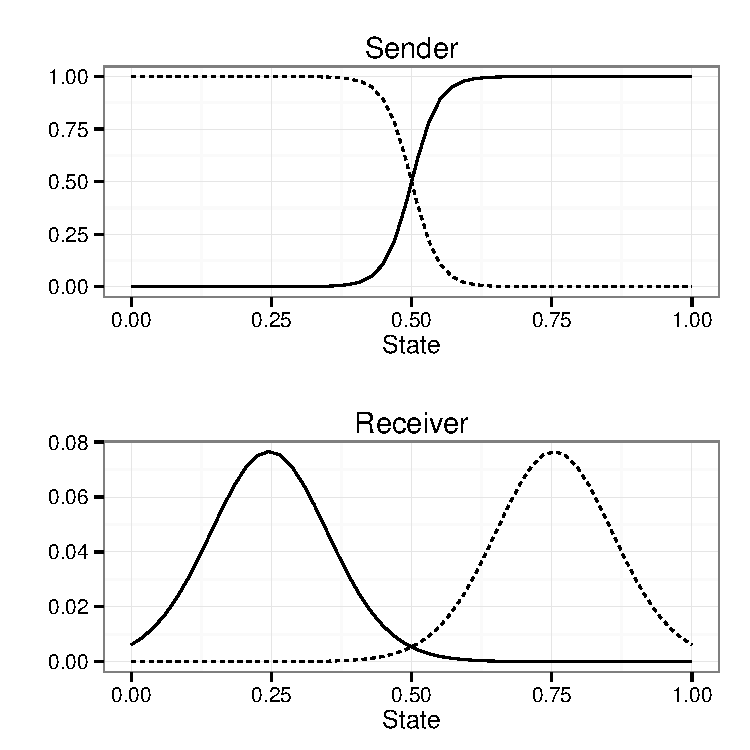
\includegraphics[width=\textwidth]{plots/exampleStratQRE_tolerance05.pdf}
    \caption{$\ns = 90$, $\lambda = 15$, $\toler = 0.5$}
    \label{fig:exampleQRE_stratsA}
  \end{subfigure}
  \hfill
  \begin{subfigure}[]{0.45\textwidth}
    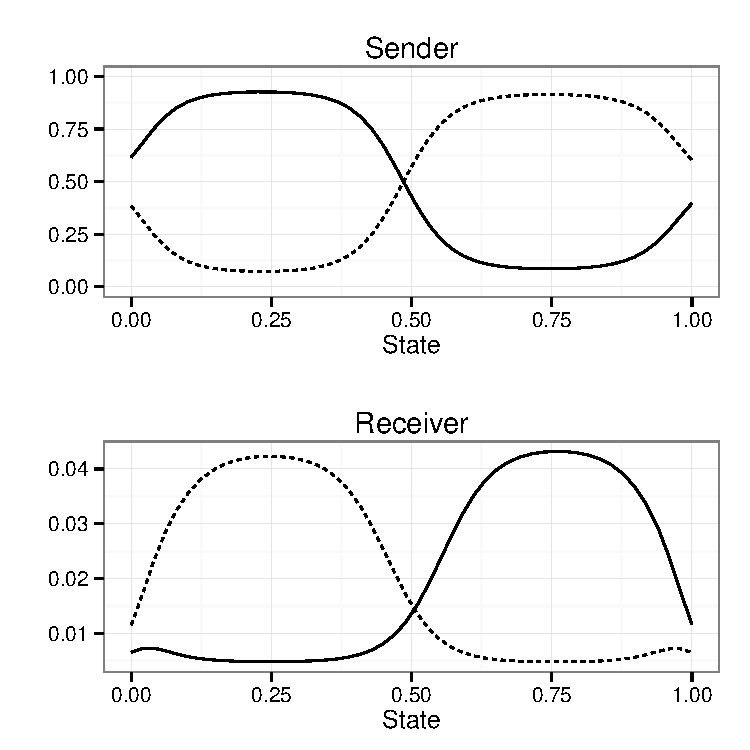
\includegraphics[width=\textwidth]{plots/exampleStratQRE_tolerance005.pdf}
    \caption{$\ns = 90$, $\lambda = 15$, $\toler = 0.05$}
    \label{fig:exampleQRE_stratsB}
  \end{subfigure}

  \caption{Examples of vague quantal response equilibria.}
  \label{fig:exampleQREs}
\end{figure}


But not all quantal response equilibria are equally plausible
explanations of vague language use, and the ones that are not suggest
that it is less plausible to think of vagueness as arising because of
errors in the computation and maximization of expected utility, as the
quantal response approach assumes, than that it arises due to
confusion of similar states, as the \rdd proposes. To see what the
problem is, we can look at cases like given in
Figure~\ref{fig:exampleQRE_stratsB}, which is the quantal response
equilibrium for a game with lower tolerance $\toler = 0.05$. Unlike
what evolves under \rdd in this case, sender strategies have vague
boundaries also towards the end of the unit intervals. Technically,
this is because quantal responses equalize message use far away from
the ``prototypical'' interpretation, not just in-between categories,
so to speak. This, in turn, is because quantal responses introduce
noise into the decision making at the level of computing or maximizing
expected utility of choices.

That this is conceptually odd shows even more clearly in a case where
the state space is intuitively unbounded, as for instance for the
property ``tall''. If the usual interpretation of a ``tall man'' peaks
at around, say, 195cm then when meeting a giant of $n$ meters speakers
would, according to the quantal response approach, be ever more
inclined to describe the giant indifferently as either ``tall'' or
``short'' the larger $n$ gets. This is because, as the distance from
the prototype increases for larger $n$, the difference between the
expected utilities of saying ``short'' or ``tall'' will converge to
zero. Whence that the quantal response approach would predict that
speakers would grow indifferent between choice of antonyms as $n$
grows, which seems weird. 

Admittedly, this argument hinges on the choice of utility
function. Still, to the extent that the chosen lower bounded utility
functions are reasonable ---and we think they are very reasonable---,
the case suggests that quantal responses are not a good model,
intuitively speaking, for why linguistic categories are
vague. Vagueness is more plausibly an effect of perceptual confusion
of similar states, than of computational errors in maximizing expected
utility.

%%% Local Variables: 
%%% mode: latex
%%% TeX-master: "paper"
%%% TeX-PDF-mode: t
%%% End:



